% ============================================================
% 电路基础实验 —— 实验二 线性电路的线性特征 实验报告
% 使用 CircuitTheory/template.tex 正式实验报告模板
% ============================================================

\documentclass[12pt]{ctexart}

% --- 宏包 ---
\usepackage{graphicx}
\usepackage{amsmath}
\usepackage{float}
\usepackage{booktabs}
\usepackage{siunitx}
\usepackage{caption}
\usepackage{subcaption}
\usepackage{enumitem}
\usepackage{fancyhdr}
\usepackage{hyperref}
\usepackage{makecell}

\sisetup{per-mode=symbol}

\graphicspath{{./figures/}{../}{./}}

\usepackage[left=2.5cm, right=2.5cm, top=2.5cm, bottom=2.5cm]{geometry}

\setlength{\jot}{6pt}
\setlength{\headheight}{15pt}
\linespread{1.5}
\setlist{nosep}

% --- 页眉页脚 ---
\pagestyle{fancy}
\fancyhead[C]{电路基础实验}
\fancyfoot[C]{\thepage}

\begin{document}

% ==================== 封面 ====================
\thispagestyle{empty}

\begin{figure}[t]
    \centering
    
\includegraphics[width=13cm]{logo1.png}
\end{figure}

\vspace*{\fill}
    \begin{center}
        \Huge\textbf{电路基础}

        \vspace{0.3cm}
        \Huge\textbf{实验报告}

        \vspace{1cm}
        \LARGE\textbf{实验二：线性电路的线性特征}
    \end{center}
\vspace*{\fill}

\begin{table}[H]
    \centering
    \large
    \begin{tabular}{ll}
    \toprule
    \textbf{课程:} & 电路基础实验 \\
    \textbf{姓名:} & 郭浩然 2024303980 \\
    \textbf{组号:} & 第7组 \\
    \textbf{时间:} & \today \\
    \bottomrule
    \end{tabular}
\end{table}

\newpage

% ==================== 正文 ====================

% (10) 实验目的
\section{实验目的}

\begin{enumerate}[label=\arabic*.]
    \item 学习 LM317 三端可调节正电压稳压器的基本原理及其作为精密恒流源的使用方法。
    \item 通过改变独立电源激励大小，验证线性电路的齐次性。
    \item 通过分别测量单独电源作用与共同作用时的响应，验证线性电路的叠加性。
\end{enumerate}

% (20) 实验原理
\section{实验原理}

\subsection{LM317 恒流源原理}

LM317 是三端可调节正电压稳压器，三个引脚分别为调整端 ADJ、输出端 \(V_{out}\) 和输入端 \(V_{in}\)。当 LM317 与取样电阻串联使用时，芯片内部基准电压可在取样电阻上形成近似恒定的压降，从而得到恒流输出。其输出电流为
\begin{equation}
    I_{out}=\frac{V_{ref}}{R}+I_{Adj}\approx\frac{1.25\,\mathrm{V}}{R}.
\end{equation}
其中 \(I_{Adj}\) 通常远小于输出电流，在实验计算中可忽略。实验中利用该恒流源为线性网络提供独立电流源激励。

\begin{figure}[H]
    \centering
    \begin{subfigure}[b]{0.32\textwidth}
        \centering
        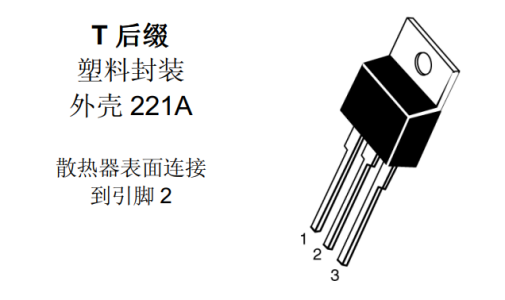
\includegraphics[width=\linewidth]{lm317_package.png}
        \caption{LM317 封装与引脚}
    \end{subfigure}
    \hfill
    \begin{subfigure}[b]{0.56\textwidth}
        \centering
        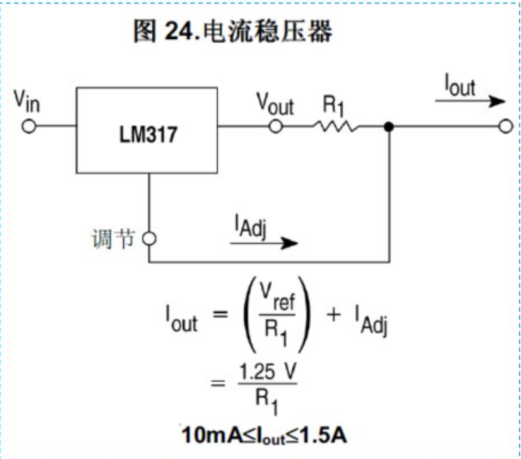
\includegraphics[width=\linewidth]{lm317_current_source_principle.png}
        \caption{LM317 恒流源接法}
    \end{subfigure}
    \caption{LM317 器件与恒流源原理}
    \label{fig:lm317}
\end{figure}

\subsection{齐次定理}

在线性电路中，当所有独立电源激励同时扩大或缩小同一倍数 \(K\) 时，各支路电压、电流响应也应扩大或缩小相同倍数。若某一响应可表示为
\begin{equation}
    y=f(x_1,x_2,\ldots,x_n),
\end{equation}
则有
\begin{equation}
    Ky=f(Kx_1,Kx_2,\ldots,Kx_n).
\end{equation}
本实验通过比较原激励与半激励条件下各支路电压、电流的测量结果，判断响应是否近似满足 \(1/2\) 倍关系。

\subsection{叠加定理}

在线性电路中，多个独立电源共同作用时，任一支路响应等于各独立电源分别单独作用时在该支路产生响应的代数和。对两个独立激励而言，有
\begin{align}
    y_1 &= f(x_1), \\
    y_2 &= f(x_2), \\
    y_1+y_2 &= f(x_1+x_2).
\end{align}
实验中分别测量电压源与电流源共同作用、电流源单独作用、电压源单独作用三种情况下的响应，并比较单独作用响应的代数和与共同作用响应之间的差异。

\subsection{Multisim 仿真}

实验电路由电压源、LM317 恒流源和电阻网络组成。电压源提供电压激励，LM317 与取样电阻构成电流源激励，电阻网络用于测量各支路电压 \(U_1,U_2,U_3\) 与电流 \(I_1,I_2,I_3\)。Multisim 仿真电路如图~\ref{fig:multisim} 所示。

\begin{figure}[H]
    \centering
    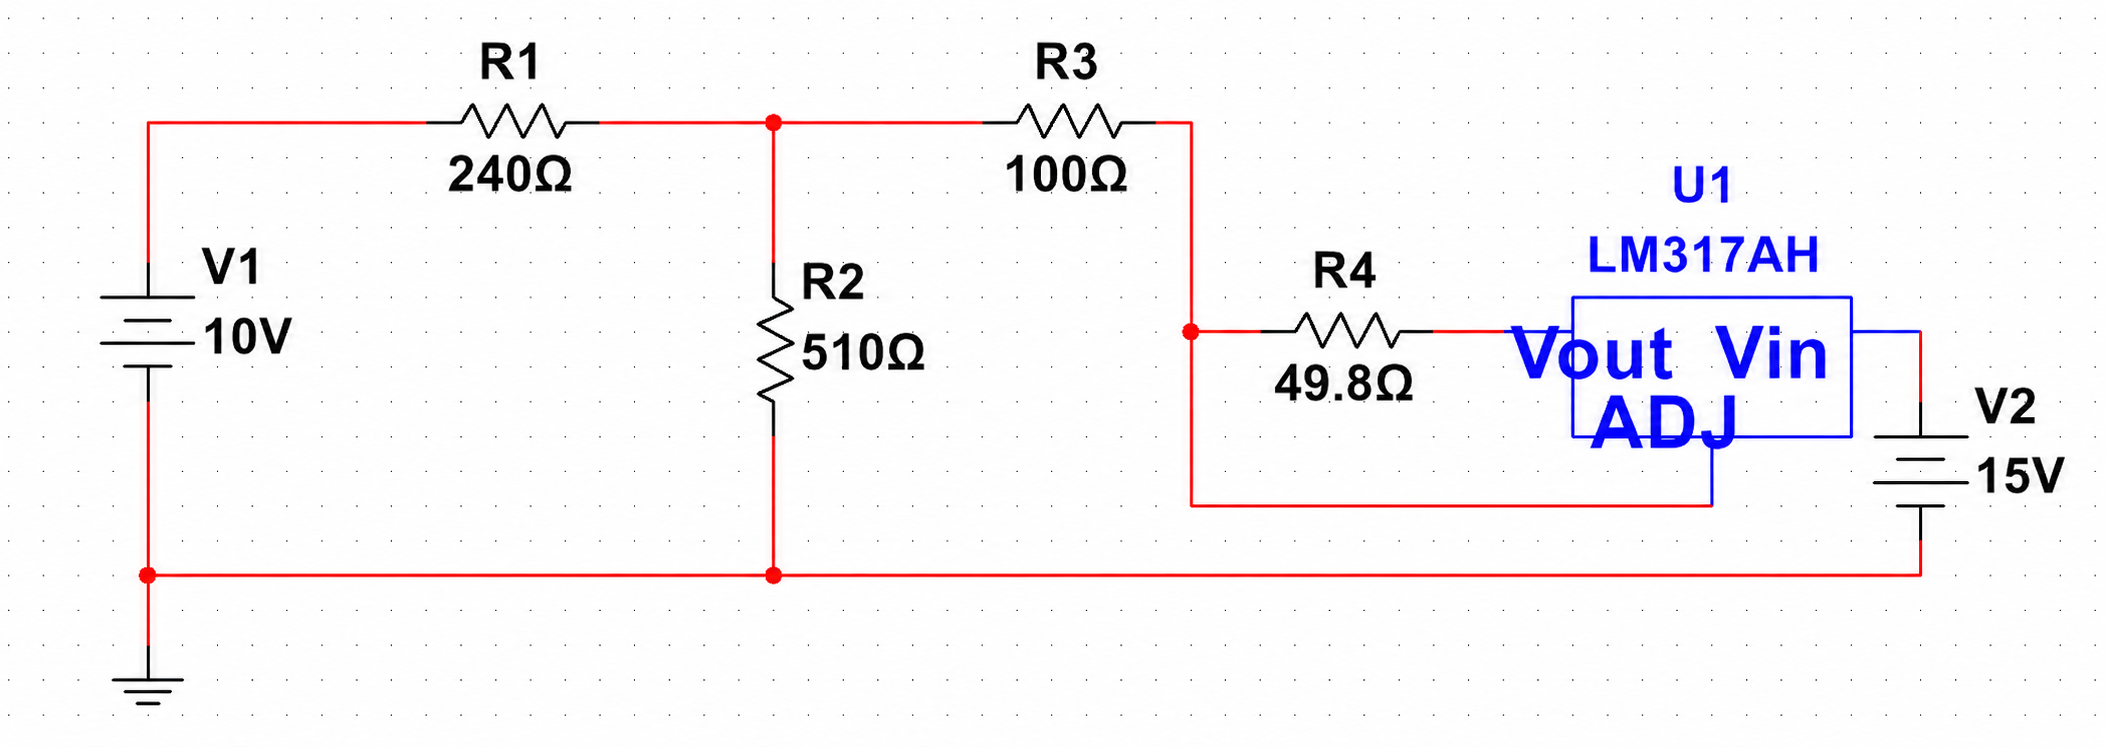
\includegraphics[width=0.92\textwidth]{experiment2_multisim_simulation.png}
    \caption{实验二 Multisim 仿真电路}
    \label{fig:multisim}
\end{figure}

% (10) 实验器件
\section{实验器件}

\begin{itemize}
    \item 面包板 \(\times 1\)
    \item 可编程直流电源 \(\times 1\)
    \item 数字万用表 \(\times 1\)
    \item LM317AH 芯片 \(\times 1\)
    \item 电阻：\(51\,\Omega\)、\(100\,\Omega\)、\(240\,\Omega\)、\(510\,\Omega\) 各 \(1\) 个
    \item 导线若干
\end{itemize}

% (10) 实验步骤
\section{实验步骤}

\begin{enumerate}[label=\arabic*.]
    \item 按实验电路图连接 LM317AH、取样电阻和直流电源，构成近似恒流源，并测量其输出电流。
    \item 根据 Multisim 仿真电路，在面包板上搭建线性电阻网络，检查电源极性、LM317 引脚和各节点连接是否正确。
    \item 设置电压源为 \(10\,\mathrm{V}\)，电流源约为 \(25.2\,\mathrm{mA}\)，测量两电源共同作用时各支路电压和电流。
    \item 将电压源和电流源同时缩小为原值的一半，测量半激励条件下的各支路响应，用于验证齐次性。
    \item 将电压源置零，即用导线短接电压源，测量电流源单独作用时的各支路响应。
    \item 将电流源置零，即断开电流源支路，测量电压源单独作用时的各支路响应。
    \item 整理实验数据，分别计算齐次性误差和叠加性误差，并分析误差来源。
\end{enumerate}

\begin{figure}[H]
    \centering
    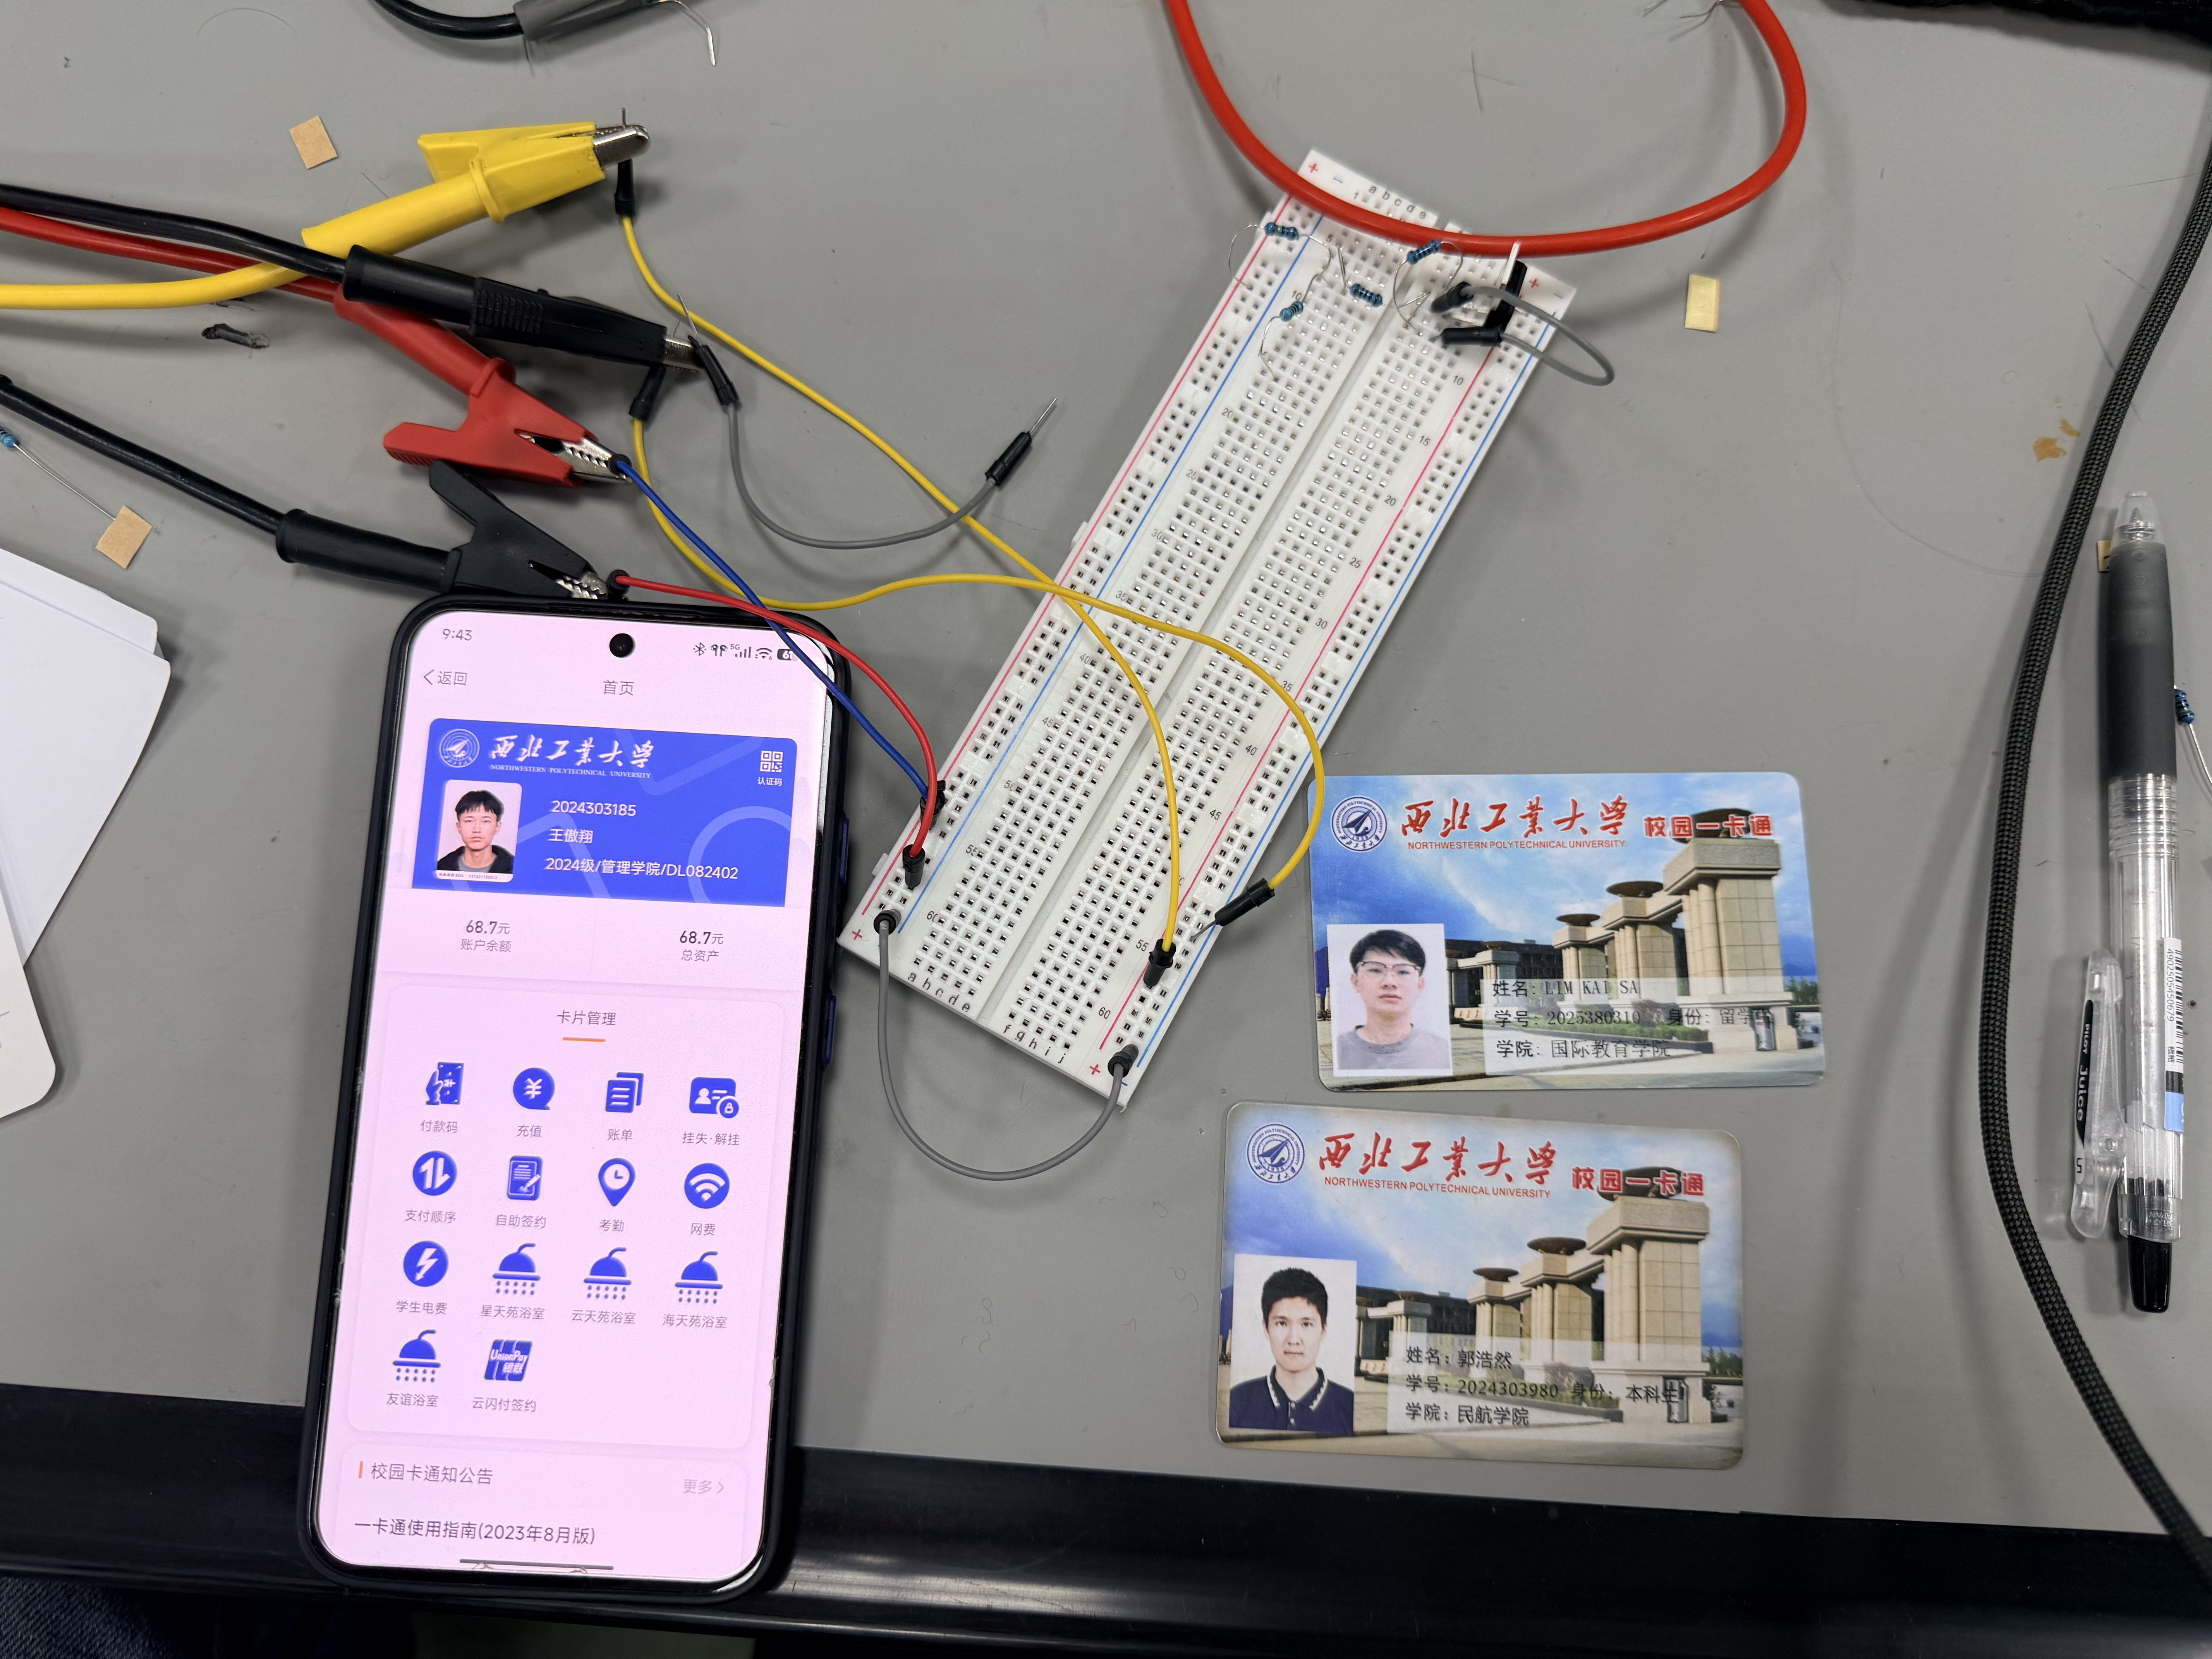
\includegraphics[width=0.82\textwidth]{experiment2_physical_circuit.jpg}
    \caption{实验二实物电路连接}
    \label{fig:physical-circuit}
\end{figure}

% (10) 实验数据
\section{实验数据}

实验原始数据记录如图~\ref{fig:raw-data} 所示。由于记录时各支路参考方向不完全统一，整理时按电路拓扑统一取：\(U_1\) 为 \(R_1\) 左端相对右端电压，\(U_2\) 为 \(R_2\) 上端相对下端电压，\(U_3\) 为 \(R_3\) 左端相对右端电压；\(I_3\) 采用原始记录中的测量电流方向。根据该方向约定，将原始记录中的读数整理为表~\ref{tab:raw-data}。

\begin{figure}[H]
    \centering
    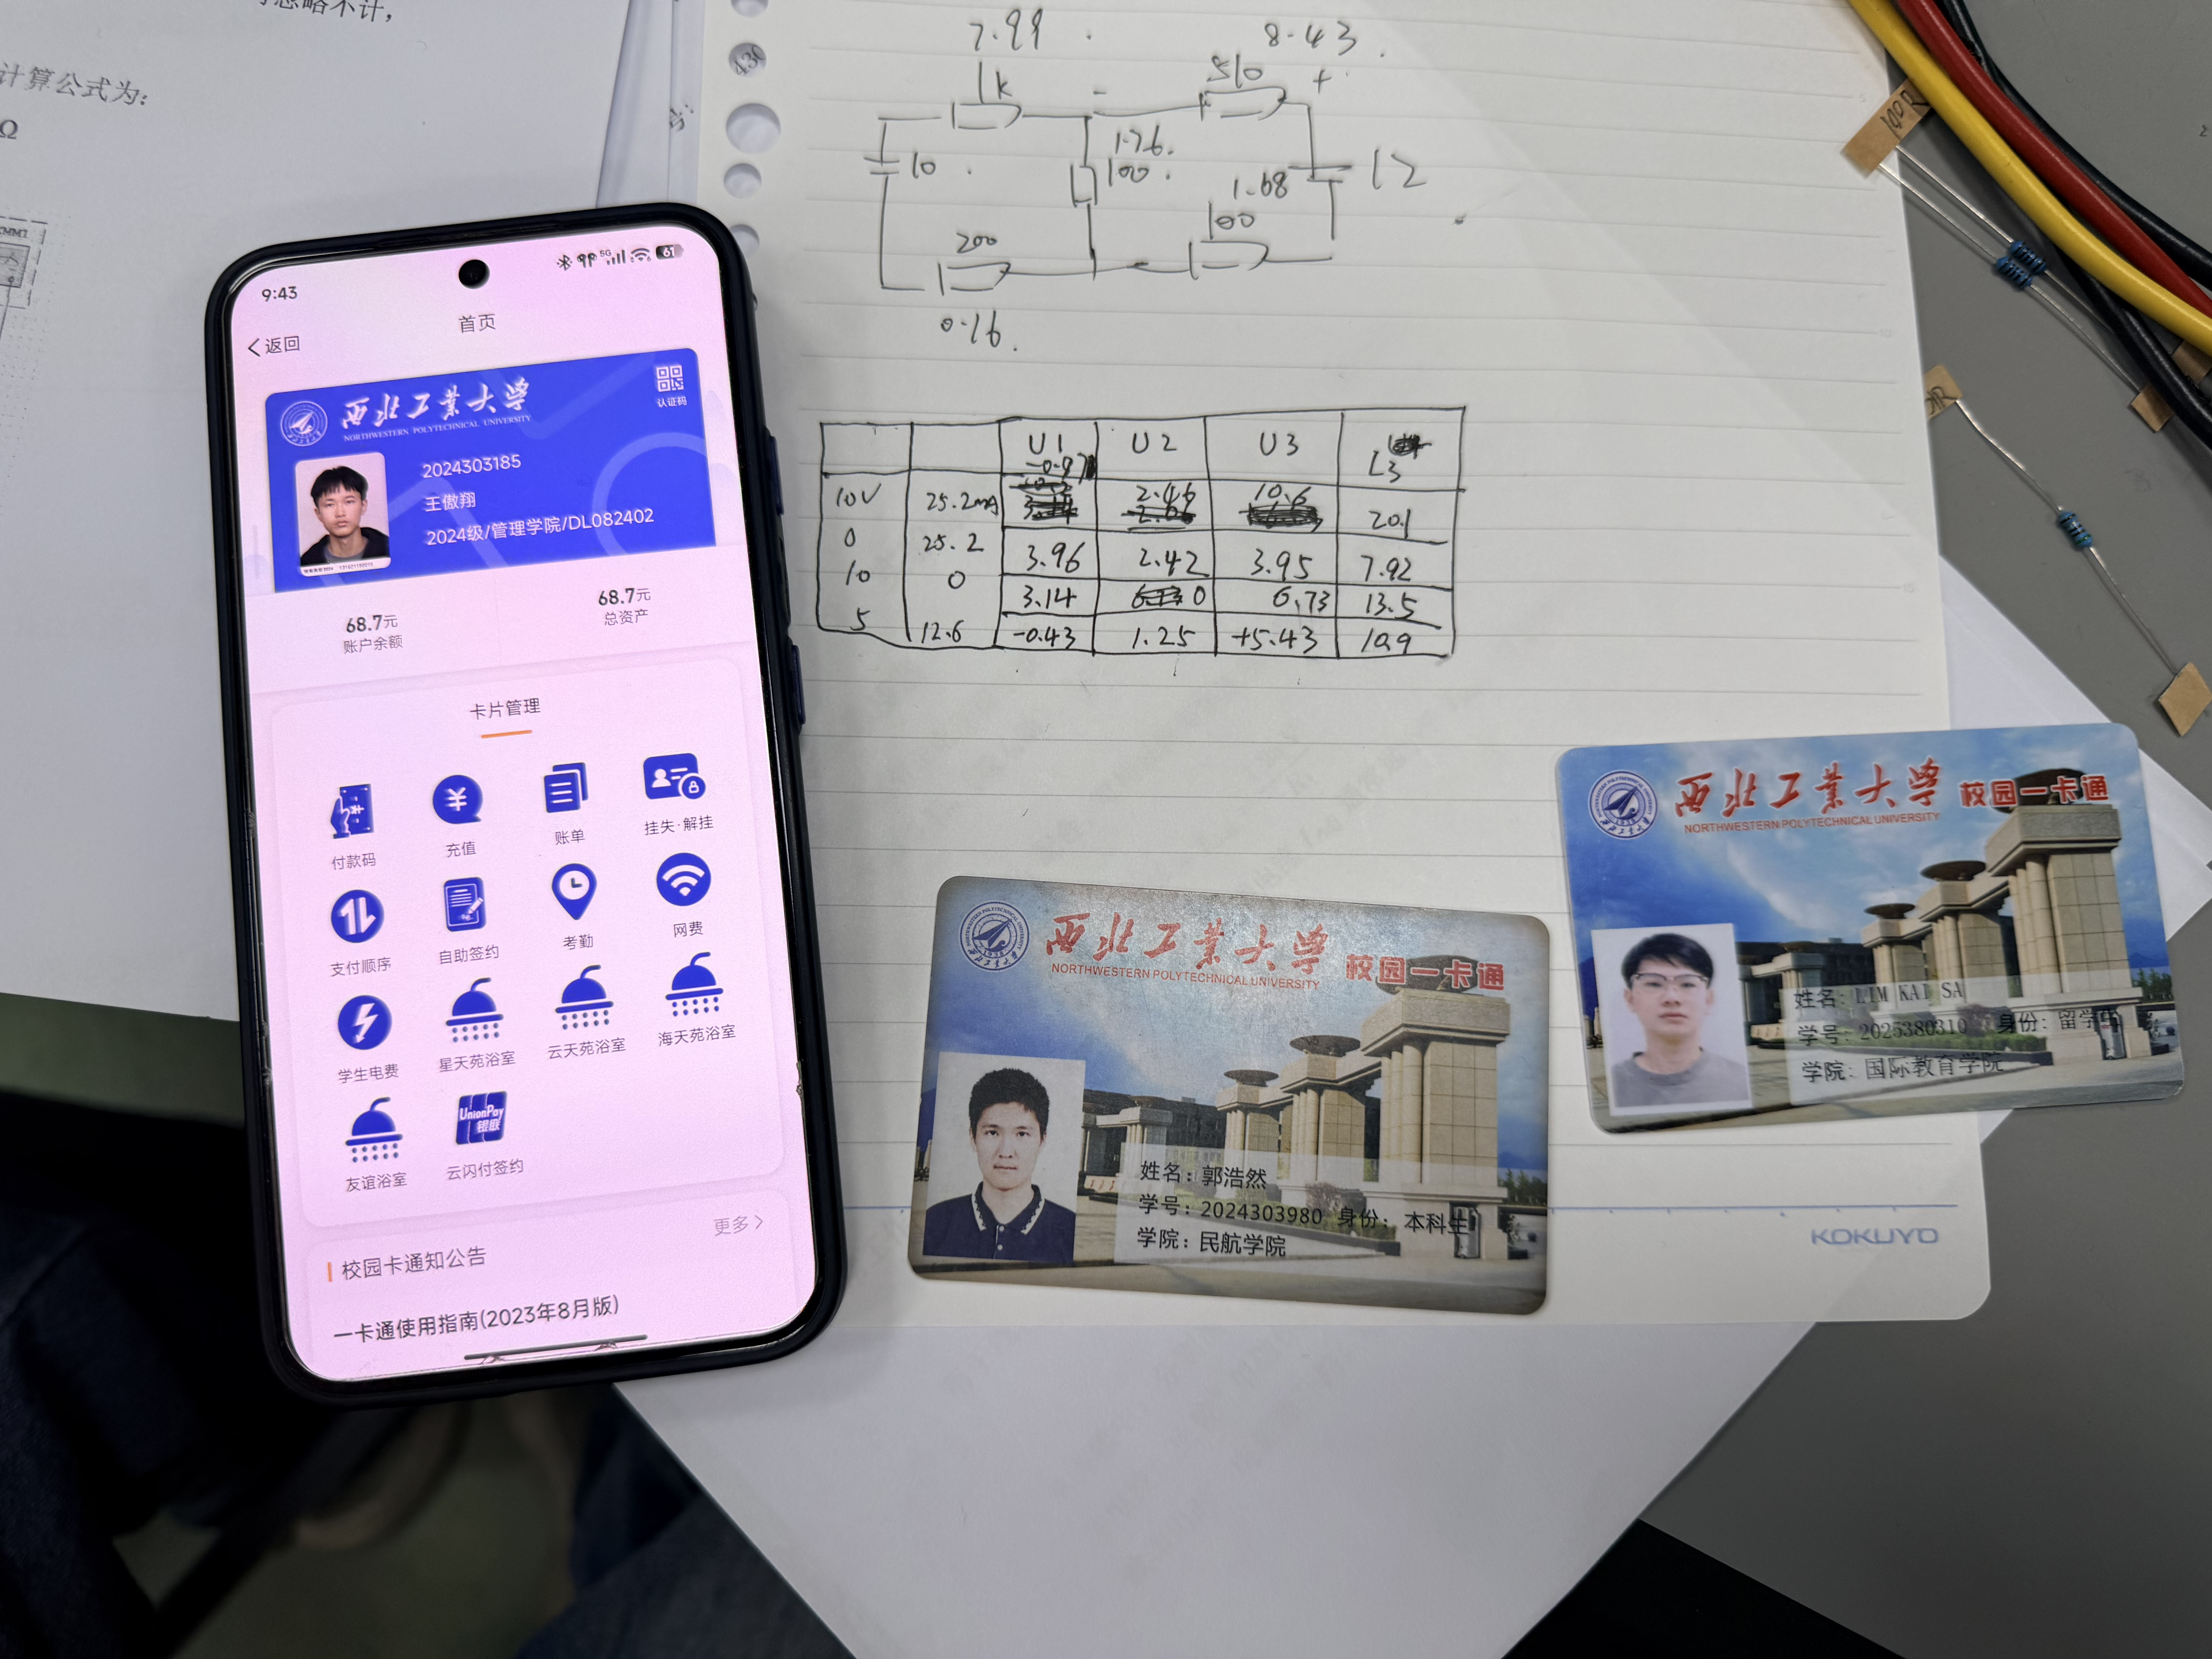
\includegraphics[width=0.82\textwidth]{experiment2_raw_data.jpg}
    \caption{实验二原始数据记录照片}
    \label{fig:raw-data}
\end{figure}

\begin{table}[H]
    \centering
    \caption{实验二原始测量数据}
    \label{tab:raw-data}
    \begin{tabular}{ccccccc}
        \toprule
        测量条件 & 电压源/V & 电流源/mA & \(U_1\)/V & \(U_2\)/V & \(U_3\)/V & \(I_3\)/mA \\
        \midrule
        共同作用 & 10 & 25.2 & -0.87 & 10.60 & -2.46 & 20.10 \\
        电流源单独作用 & 0 & 25.2 & -3.96 & 3.95 & -2.42 & 7.92 \\
        电压源单独作用 & 10 & 0 & 3.14 & 6.73 & 0 & 13.50 \\
        半激励 & 5 & 12.6 & -0.43 & 5.43 & -1.25 & 10.90 \\
        \bottomrule
    \end{tabular}
\end{table}

% (20) 数据分析
\section{数据分析}

\subsection{实验数据与理论公式对比}

齐次性要求当所有独立激励同时缩小为原来的 \(1/2\) 时，电路中各支路电压和电流也应缩小为原来的 \(1/2\)。各参数误差按
\begin{equation}
    \Delta=\left|x_{\frac{1}{2}\text{激励}}-\frac{x_{\text{原激励}}}{2}\right|
\end{equation}
计算。根据表~\ref{tab:homogeneity}，\(U_1\)、\(U_2\)、\(U_3\) 的齐次性误差分别为 \(0.005\,\mathrm{V}\)、\(0.13\,\mathrm{V}\)、\(0.02\,\mathrm{V}\)，相对于对应电压读数较小；\(I_3\) 的误差为 \(0.85\,\mathrm{mA}\)，相对电流读数也处于可接受范围内。因此，当电压源由 \(10\,\mathrm{V}\) 变为 \(5\,\mathrm{V}\)、电流源由 \(25.2\,\mathrm{mA}\) 变为 \(12.6\,\mathrm{mA}\) 时，电路响应基本按相同比例缩小，说明该电路的齐次性得到验证。

\begin{table}[H]
    \centering
    \caption{齐次性验证数据}
    \label{tab:homogeneity}
    \begin{tabular}{ccccc}
        \toprule
        参数 & 原激励实测值 & 原激励实测值/2 & 半激励实测值 & 绝对误差 \\
        \midrule
        \(U_1\)/V & -0.87 & -0.435 & -0.43 & 0.005 \\
        \(U_2\)/V & 10.60 & 5.30 & 5.43 & 0.13 \\
        \(U_3\)/V & -2.46 & -1.23 & -1.25 & 0.02 \\
        \(I_3\)/mA & 20.10 & 10.05 & 10.90 & 0.85 \\
        \bottomrule
    \end{tabular}
\end{table}

\subsection{不同测量方法比较}

叠加性要求电压源和电流源共同作用时的响应等于二者单独作用时响应的代数和。各参数误差按
\begin{equation}
    \Delta=\left|x_{\text{共同作用}}-\left(x_{\text{电流源单独}}+x_{\text{电压源单独}}\right)\right|
\end{equation}
计算。由表~\ref{tab:superposition} 可知，\(U_1\)、\(U_2\)、\(U_3\) 的共同作用实测值与两个单独作用实测值的代数和分别相差 \(0.05\,\mathrm{V}\)、\(0.08\,\mathrm{V}\)、\(0.04\,\mathrm{V}\)，吻合程度较好。\(I_3\) 的叠加误差为 \(1.32\,\mathrm{mA}\)，大于电压项误差，主要可能来自电流档串入测量时对支路状态的扰动、读数方向不完全一致以及恒流源输出波动。总体来看，共同作用响应与单独作用响应代数和接近，线性电路的叠加性得到验证。

\begin{table}[H]
    \centering
    \caption{叠加性验证数据}
    \label{tab:superposition}
    \begin{tabular}{cccccc}
        \toprule
        参数 & 共同作用 & 电流源单独 & 电压源单独 & 单独作用代数和 & 绝对误差 \\
        \midrule
        \(U_1\)/V & -0.87 & -3.96 & 3.14 & -0.82 & 0.05 \\
        \(U_2\)/V & 10.60 & 3.95 & 6.73 & 10.68 & 0.08 \\
        \(U_3\)/V & -2.46 & -2.42 & 0 & -2.42 & 0.04 \\
        \(I_3\)/mA & 20.10 & 7.92 & 13.50 & 21.42 & 1.32 \\
        \bottomrule
    \end{tabular}
\end{table}

\subsection{误差来源分析}

实验误差主要来自以下方面：
\begin{enumerate}[label=\arabic*.]
    \item 电阻存在标称误差，实际阻值与标称值不完全一致，导致理论计算值与实测值存在偏差。
    \item LM317 恒流源输出电流会受输入电压、负载压降、调整端电流和芯片温升影响，实际输出电流存在波动。
    \item 数字万用表读数存在分辨率误差，测量电压和电流时读数也可能有小幅变化。
    \item 面包板和导线接触电阻会引入附加压降，接线松动也会影响测量结果。
    \item 电源输出电压和电流源实际输出值与设定值之间存在微小偏差。
\end{enumerate}

通过对原激励、半激励、单独电源作用和共同作用条件下各支路响应的测量与比较，可以验证线性电路的齐次性和叠加性。在统一参考方向后，半激励响应与原激励响应的一半基本一致，共同作用响应也与两个单独作用响应的代数和基本一致。实验误差在合理范围内，实验结果与线性电路理论相符。

\end{document}
